\section{Detailed Explanation}
    \subsection{Seven Explanatory Criterion}
        \indent The explanatory criterion\cite{tintarev2007survey} (see table \ref{table:1}), originally proposed by Nava Tintarev and Judith Masthoff, 
        are mostly used when considering to design the explanation of a recommender system. 

        \begin{table}[ht] 
            % ht used to attach the table to the position approximately where they are wrote here
            \centering
            \begin{tabular}{ | m{8em} | m{4cm} | }
            \hline
            %  \bfseries used to bold the header
            \bfseries Aim & \bfseries Definition\\ [0.5ex] 
            \hline\hline
            Transparency & Explain how the system works\\ 
            \hline
            Scrutability & Allow users to tell the system it is wrong\\ 
            \hline
            Trust & Increase users' confidence in the system\\ 
            \hline
            Effectiveness & Help users make good decisions\\ 
            \hline
            Persuasiveness & Convince users to try\\ 
            \hline
            Efficiency & Help users make decisions faster\\ 
            \hline
            Satisfaction & Increase the ease of use or enjoyment\\ 
            \hline
            \end{tabular}
            \caption{Explanatory criteria and their definitions}
            \label{table:1}
        \end{table}
        \indent Although they have different names in different researches. For example, 
        Mohammed Z.Taie call them explanation attributes\cite{al2013explanations},
        which represent the benefits explanations provide to recommender systems and Fatih Gedikli call them quality factors, 
        which he used to evaluate different explanation types in his study\cite{gedikli2014should}.
        They have the same purpose, that is, to make the system more understandable by users.
        These criterion are listed here as follows:
        
        \begin{enumerate}
            \item \textbf{Transparency:} TODO:// write the intro
            \item \textbf{Scrutability:} TODO:// write the intro
            \item \textbf{Trust:} TODO:// write the intro
            \item \textbf{Effectiveness:} TODO:// write the intro
            \item \textbf{Persuasiveness:} TODO:// write the intro
            \item \textbf{Efficiency:} TODO:// write the intro
            \item \textbf{Satisfaction:} TODO:// write the intro
        \end{enumerate}
    \subsection{Examples of Detailed Explanation}
        An example of explanation in amazon.com.
        TODO: (Write Analysis based on seven explanatory criterion) 
        \begin{figure}[H]
            \centering
            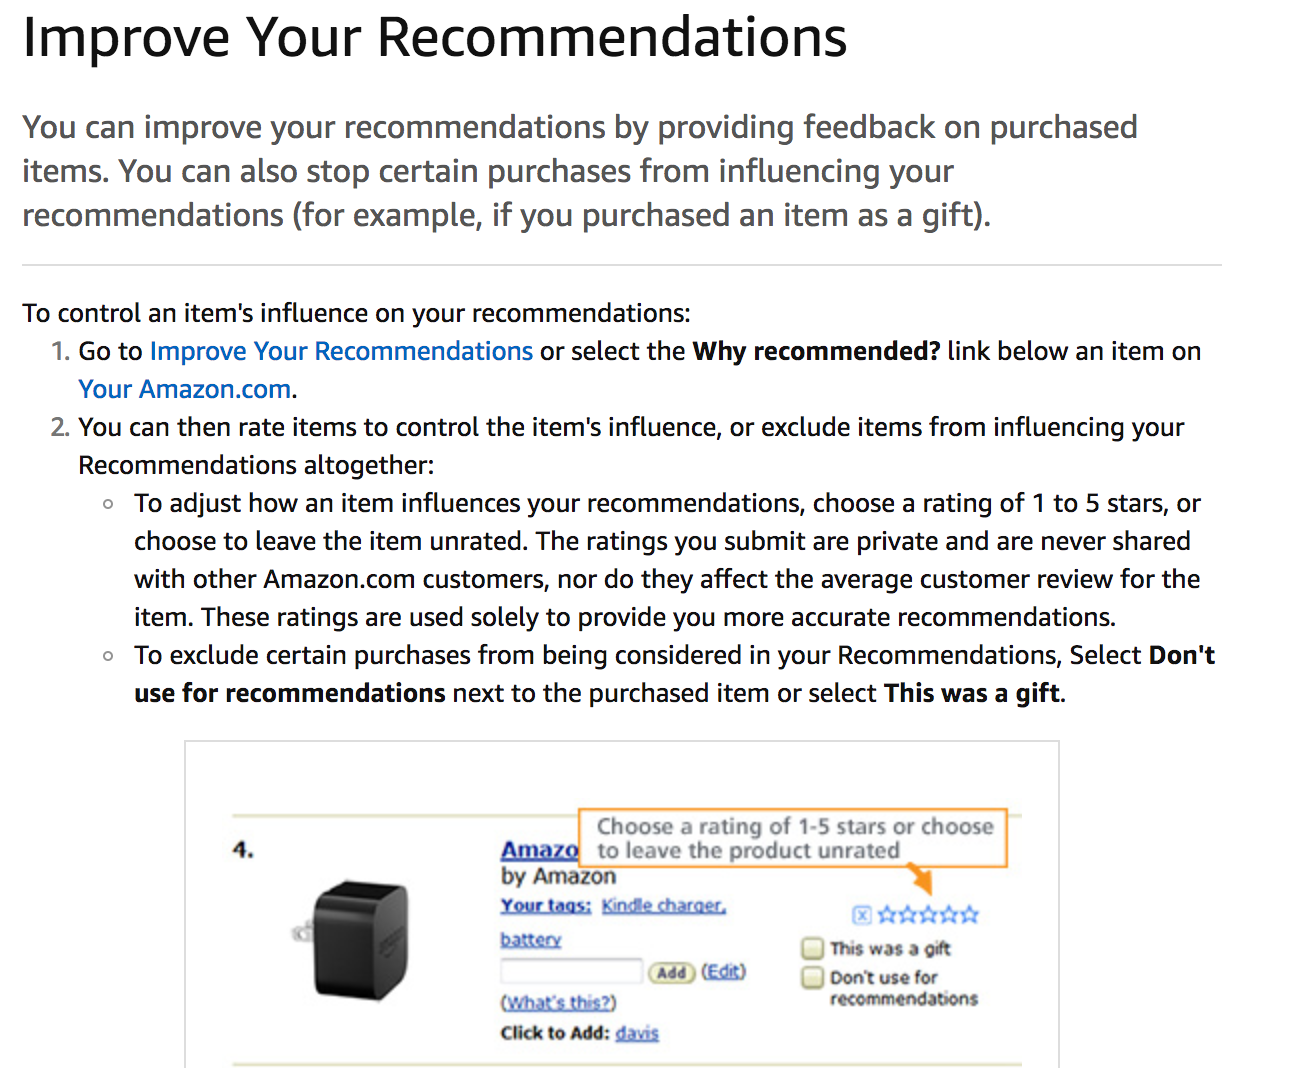
\includegraphics[width=0.5\textwidth]{img/amazon1}
            \caption{Amazon}
            \label{fig:amazon1}
        \end{figure}
        An example of explanation of Google Ads.
        TODO:  (Write Analysis based on seven explanatory criterion) 
        \begin{figure}[H]
            \centering
            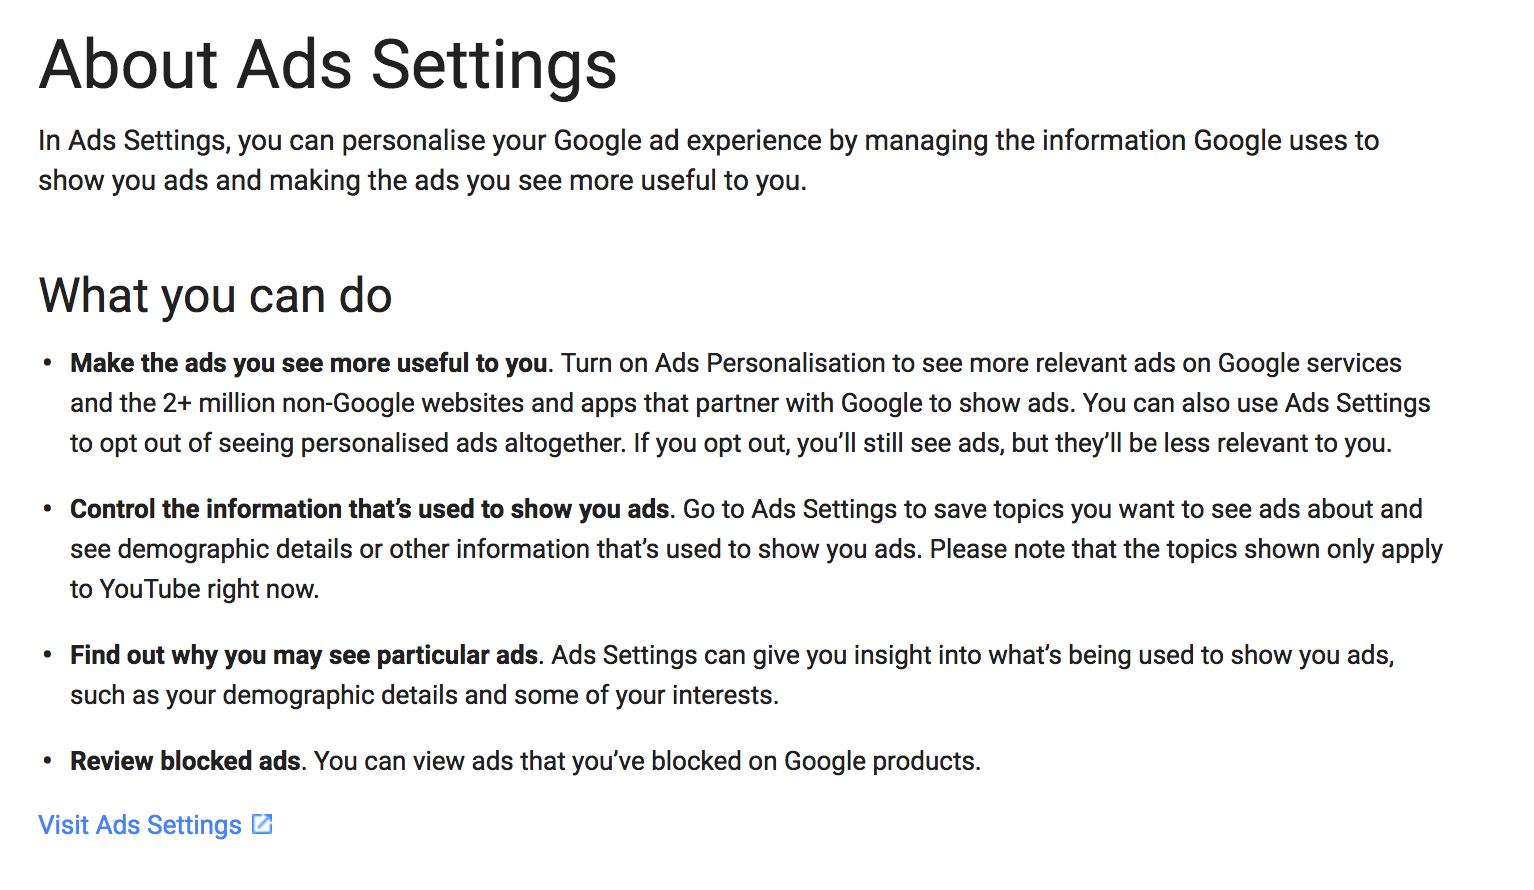
\includegraphics[width=0.5\textwidth]{img/google1}
            \caption{Google}
            \label{fig:google1}
        \end{figure}
\section{Short Explanation}
    However, in some scenario, a brief explanation is more suitable, for example, driving in a car
    (why: users have limited attention resource)
    We can not take all seven explanatory criterion into consideration.
    How to extract a kind of standards.
    
    \subsection{Possible Criterion for Short Explanation}

    \subsection{Examples of Short Explanation}
        Example1: Explanations in Proactive Recommender Systems in Automotive Scenarios \cite{bader122011explanations}
        \textbf{Extract two criterion out of seven explanatory criterion: Persuasiveness and Efficiency.}

        Example2: Why did my car just do that? Explaining semi-autonomous driving actions to improve driver understanding, trust, and performance\cite{koo2015did}
        \textbf{Extract two types (what and how)based on question types from Intelligent Toolkit} \cite{Brian2010toolkit, lim2011design}
